% Options for packages loaded elsewhere
\PassOptionsToPackage{unicode}{hyperref}
\PassOptionsToPackage{hyphens}{url}
%
\documentclass[
  12pt,
]{article}
\usepackage{lmodern}
\usepackage{amsmath}
\usepackage{ifxetex,ifluatex}
\ifnum 0\ifxetex 1\fi\ifluatex 1\fi=0 % if pdftex
  \usepackage[T1]{fontenc}
  \usepackage[utf8]{inputenc}
  \usepackage{textcomp} % provide euro and other symbols
  \usepackage{amssymb}
\else % if luatex or xetex
  \usepackage{unicode-math}
  \defaultfontfeatures{Scale=MatchLowercase}
  \defaultfontfeatures[\rmfamily]{Ligatures=TeX,Scale=1}
\fi
% Use upquote if available, for straight quotes in verbatim environments
\IfFileExists{upquote.sty}{\usepackage{upquote}}{}
\IfFileExists{microtype.sty}{% use microtype if available
  \usepackage[]{microtype}
  \UseMicrotypeSet[protrusion]{basicmath} % disable protrusion for tt fonts
}{}
\makeatletter
\@ifundefined{KOMAClassName}{% if non-KOMA class
  \IfFileExists{parskip.sty}{%
    \usepackage{parskip}
  }{% else
    \setlength{\parindent}{0pt}
    \setlength{\parskip}{6pt plus 2pt minus 1pt}}
}{% if KOMA class
  \KOMAoptions{parskip=half}}
\makeatother
\usepackage{xcolor}
\IfFileExists{xurl.sty}{\usepackage{xurl}}{} % add URL line breaks if available
\IfFileExists{bookmark.sty}{\usepackage{bookmark}}{\usepackage{hyperref}}
\hypersetup{
  pdftitle={Supplementary Information},
  hidelinks,
  pdfcreator={LaTeX via pandoc}}
\urlstyle{same} % disable monospaced font for URLs
\usepackage[margin=1in]{geometry}
\usepackage{longtable,booktabs}
\usepackage{calc} % for calculating minipage widths
% Correct order of tables after \paragraph or \subparagraph
\usepackage{etoolbox}
\makeatletter
\patchcmd\longtable{\par}{\if@noskipsec\mbox{}\fi\par}{}{}
\makeatother
% Allow footnotes in longtable head/foot
\IfFileExists{footnotehyper.sty}{\usepackage{footnotehyper}}{\usepackage{footnote}}
\makesavenoteenv{longtable}
\usepackage{graphicx}
\makeatletter
\def\maxwidth{\ifdim\Gin@nat@width>\linewidth\linewidth\else\Gin@nat@width\fi}
\def\maxheight{\ifdim\Gin@nat@height>\textheight\textheight\else\Gin@nat@height\fi}
\makeatother
% Scale images if necessary, so that they will not overflow the page
% margins by default, and it is still possible to overwrite the defaults
% using explicit options in \includegraphics[width, height, ...]{}
\setkeys{Gin}{width=\maxwidth,height=\maxheight,keepaspectratio}
% Set default figure placement to htbp
\makeatletter
\def\fps@figure{htbp}
\makeatother
\setlength{\emergencystretch}{3em} % prevent overfull lines
\providecommand{\tightlist}{%
  \setlength{\itemsep}{0pt}\setlength{\parskip}{0pt}}
\setcounter{secnumdepth}{5}
\usepackage{rotating}
\usepackage{setspace}
\usepackage{booktabs}
\usepackage{longtable}
\usepackage{array}
\usepackage{multirow}
\usepackage{wrapfig}
\usepackage{float}
\usepackage{colortbl}
\usepackage{pdflscape}
\usepackage{tabu}
\usepackage{threeparttable}
\usepackage{threeparttablex}
\usepackage[normalem]{ulem}
\usepackage{makecell}
\usepackage{xcolor}
\ifluatex
  \usepackage{selnolig}  % disable illegal ligatures
\fi
\newlength{\cslhangindent}
\setlength{\cslhangindent}{1.5em}
\newlength{\csllabelwidth}
\setlength{\csllabelwidth}{3em}
\newenvironment{CSLReferences}[2] % #1 hanging-ident, #2 entry spacing
 {% don't indent paragraphs
  \setlength{\parindent}{0pt}
  % turn on hanging indent if param 1 is 1
  \ifodd #1 \everypar{\setlength{\hangindent}{\cslhangindent}}\ignorespaces\fi
  % set entry spacing
  \ifnum #2 > 0
  \setlength{\parskip}{#2\baselineskip}
  \fi
 }%
 {}
\usepackage{calc}
\newcommand{\CSLBlock}[1]{#1\hfill\break}
\newcommand{\CSLLeftMargin}[1]{\parbox[t]{\csllabelwidth}{#1}}
\newcommand{\CSLRightInline}[1]{\parbox[t]{\linewidth - \csllabelwidth}{#1}\break}
\newcommand{\CSLIndent}[1]{\hspace{\cslhangindent}#1}

\title{Supplementary Information}
\author{}
\date{\vspace{-2.5em}}

\begin{document}
\maketitle

{
\setcounter{tocdepth}{2}
\tableofcontents
}
\pagenumbering{gobble}
\pagenumbering{arabic}
\doublespacing

\hypertarget{testing-robustness-of-l2-racial-estimates}{%
\section*{Testing Robustness of L2 Racial Estimates}\label{testing-robustness-of-l2-racial-estimates}}
\addcontentsline{toc}{section}{Testing Robustness of L2 Racial Estimates}

As discussed in the body of this manuscript, our municipality-level racial estimates are constructed by aggregating up from individual-level records provided by L2. Because L2 uses statistical modeling to infer voters' race---not self-reported information---there is potential room for error in these estimates.

While most states in the country do not ask voters to self-report their race when they register to vote, a handful \emph{do} collect this information. The raw voter files in these states, then, include true individual-level information about the racial makeup of the electorate.

To test the validity of the L2 records, we use the L2 estimates and self-reported race from the raw voter files in Florida, Georgia, and North Carolina. We use both sets of data to estimate the Black share of the electorate in each municipality used in the body of this paper. Comparing the ``estimated'' share Black from L2 to the ``real'' share Black from the voter file gives us a good sense of how well our approach works in these states.

In Table \ref{tab:mae} we present the mean average error (MAE) of the L2 estimates aggregated up to the municipality level. The MAE is commonly used to measure how different an estimated number is from its real value. Because it seems possible that these errors could be larger in smaller municipalities, we present the MAE for each quartile of the set of municipalities as measured by population, as well as the overall MAE.

\begin{singlespace}
\begin{table}[H]

\caption{\label{tab:mae-chunck}\label{tab:mae} MAE of L2 Municipality Estimates (Florida, Georgia, North Carolina)}
\centering
\begin{tabular}[t]{ccccc}
\toprule
Bottom Quartile & Second Quartile & Third Quartile & Fourth Quartile & Overall\\
\midrule
1.08\% & 1.38\% & 1.36\% & 1.48\% & 1.32\%\\
\bottomrule
\end{tabular}
\end{table}
\end{singlespace}

Table \ref{tab:mae} makes clear that for no group of municipalities does the MAE exceed 1.5\%. Although this robustness check is limited to just 3 states, the available evidence indicates that aggregating from individual-level racial estimates in the L2 data to municipality-level demographics of the electorate does not result in unacceptable biases.

\hypertarget{regression-table-for-survey-data}{%
\section*{Regression Table for Survey Data}\label{regression-table-for-survey-data}}
\addcontentsline{toc}{section}{Regression Table for Survey Data}

Here we present the regression table reported in the national survey data section of the manuscript. In model 1 we test whether personal or proximal contact with a police stop is differentially associated with turnout for Black and non-Black respondents. In this model, \emph{Stopped in Past 12 Months} captures the relationship between police stops and non-Black respondents; \emph{Stopped in Past 12 Months × Black} tests whether this relationship is different for Black respondents.

Models 2, 3, and 4 test whether the relationship is different for other non-white groups. Finally, model 5 tests the relationship between turnout and a historical arrest.

\begin{singlespace}
\input{"../temp/anes_clean.tex"}
\end{singlespace}

Model 1 in Table \ref{tab:anes-reg} shows that Black individuals who had been stopped by the police (or had a family member stopped) in the preceding 12 months were 9 percentage points more likely to vote in 2020, other things equal; they were not related to turnout for non-Black respondents. Police stops are not, however, associated with different turnout effects for other non-white groups. Moreover, as discussed in the body of the paper, historical arrests were uniformly associated with a decrease in turnout of 4 percentage points for Black and non-Black respondents alike.

\hypertarget{regression-table-for-2018-cross-sectional-municipality-model}{%
\section*{Regression Table for 2018 Cross-Sectional Municipality Model}\label{regression-table-for-2018-cross-sectional-municipality-model}}
\addcontentsline{toc}{section}{Regression Table for 2018 Cross-Sectional Municipality Model}

In Table \ref{tab:cog-cross-reg} we present the full results of the econometric used to test the cross-sectional relationship between per-capita fees and fines, and 2018 municipal turnout. The table shows that a doubling of the fees and fines collected per capita is associated with a 0.3 percentage point reduction in overall turnout. That same doubling, however, is associated with a 0.4 percentage point \emph{increase} in the Black turnout. While these point estimates are quite small, it is worth keeping in mind that the range of fees and fines per capita is very wide. The interquartile ranges of fees and fines per capita stretches from \$1.96 to \$20.63---a more than ten-fold increase.

\begin{singlespace}
\input{"../temp/cog_cross_clean.tex"}
\end{singlespace}

\hypertarget{administrative-matching-robustness-check}{%
\section*{Administrative Matching Robustness Check}\label{administrative-matching-robustness-check}}
\addcontentsline{toc}{section}{Administrative Matching Robustness Check}

Our models exploring the turnout effects of traffic stops in Hillsborough County, Florida, require that we merge administrative records using the identifiers in the data. This runs the risk of identifying false positives. To test the prevalence of false positives in our administrative matching procedure, we use the test developed by \protect\hyperlink{ref-Meredith2014}{Meredith and Morse} (\protect\hyperlink{ref-Meredith2014}{2014}). By systematically permuting the birth dates in one set of records, we can see whether false positive matches are a major concern. In Table \ref{tab:change-dobs} we begin by merging all names and dates of birth in the traffic stop data with the names and dates of birth in the Hillsborough County registered voter file. We then add and subtract 35 days from the birth dates in the traffic stop data. If there are no false positives, these records should match with no records from the registered voter file.

\begin{singlespace}
\begin{table}[H]

\caption{\label{tab:shift-dobs-chunk}\label{tab:change-dobs} Results of Shifting Birthdates}
\centering
\begin{tabular}[t]{cc}
\toprule
Group & \makecell[c]{Number of Matches Between\\Traffic Stop and Voter File Records}\\
\midrule
Actual Birthdate & 263,152\\
Birthdate + 35 Days & 78\\
Birthdate - 35 Days & 60\\
\bottomrule
\end{tabular}
\end{table}
\end{singlespace}

As the table makes clear, more than a quarter-million registered voters in Hillsborough County match at least one record in the traffic stop database when merging by first and last name, and date of birth. Once we permute the birth dates, however, the match rate drops dramatically---to 60 or 78, depending on how these dates of birth are permuted. This translates into a false positive rate of roughly 0.03 percent. We consider this rate of false positives too low to meaningfully impact our results.

\hypertarget{sensitivity-to-narrower-windows}{%
\section*{Sensitivity to Narrower Windows}\label{sensitivity-to-narrower-windows}}
\addcontentsline{toc}{section}{Sensitivity to Narrower Windows}

In the individual-level section of this manuscript, voters stopped in the 2 years prior to an election are considered treated, and we draw our controls from the voters stopped 2 years after the election. It is perhaps the case that this large window results in implausible matches; under this design, a treated voter stopped in December of 2012 could draw a control not stopped until October of 2016. Voters stopped nearly 4 years apart from one another might differ in meaningful ways that our matching models cannot capture.

Here, we re-run our matching process on a variety of different windows around the elections. In the most conservative approach, we force voters stopped in the month before an election to match with voters stopped in the month after the election; we then gradually relax this assumption by allowing voters stopped in the 2 months before the election to match to those stopped in the 2 months afterwards, etc.

Figure \ref{fig:rob-window} shows that our overall treatment effect is remarkably consistent regardless of the size of the window drawn around the election. As we expand the window, we gain more treated voters (and treated voters have a larger pool of potential controls). As such, the confidence interval shrinks, but the overall effect is clearly robust to very strict assumptions. In each case, we are re-estimating our primary models in which the covariates used in the matching exercise are also included in the econometric model.

\begin{figure}[H]

{\centering 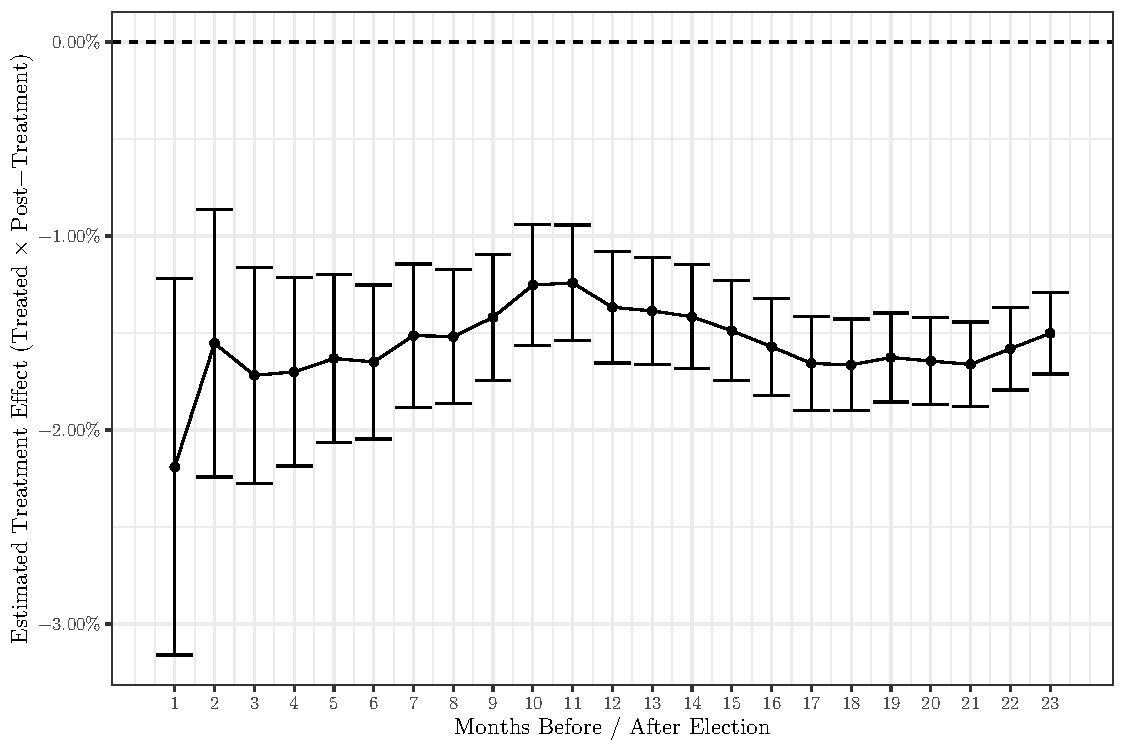
\includegraphics{si_files/figure-latex/windows-1} 

}

\caption{\label{fig:rob-window}Estimated Treatment Effect for Different Treatment Windows}\label{fig:windows}
\end{figure}

\newpage

\hypertarget{references}{%
\section*{References}\label{references}}
\addcontentsline{toc}{section}{References}

\hypertarget{refs}{}
\begin{CSLReferences}{1}{0}
\leavevmode\hypertarget{ref-Meredith2014}{}%
Meredith, Marc, and Michael Morse. 2014. {``Do {Voting Rights Notification Laws Increase Ex}-{Felon Turnout}?''} \emph{The ANNALS of the American Academy of Political and Social Science} 651 (1): 220--49. \url{https://doi.org/10.1177/0002716213502931}.

\end{CSLReferences}

\end{document}
